\documentclass[12pt,a4paper,UTF8]{ctexart}
\title{《 计算机图形学》试题A}
\author{li qiming}
\date{\today}

\usepackage{textcomp}  %允许\textdegree宏,用于显示特殊符号,如角度360°。

\usepackage{amsmath}  %数学公式

\usepackage{graphicx}  %插入图片

\usepackage{setspace}  %设置行距
\onehalfspacing  %1.5倍行距
%\addtolength{\parskip}{.4em} 设置段间距

\usepackage{geometry}  %设置页边距
\geometry{a4paper,left=3.18cm,right=3.18cm,top=2.54cm,bottom=2.54cm}
%\geometry{a4paper,scale=0.8}

%\usepackage{indentfirst}  %首行缩进
%\setlength{\parindent}{2em}  %2字符\indent缩进\noindent不缩进

\usepackage{fancyhdr}  %设置页眉页脚
\pagestyle{fancy}
\lhead{\leftmark}  %\leftmark章标题\rightmark节标题
\chead{}
\rhead{\today}
\lfoot{}
\cfoot{\thepage}
\rfoot{}

\begin{document}
	\maketitle
	\tableofcontents  %插入目录
	~\\  %插入空行
	\begin{center}  %居中
		\par {\bfseries 武汉大学《 计算机图形学》期末考试试题,满分100分}  %加黑
		\par {\bfseries 简答题共5小题,每题6分,共30分}
		\par {\bfseries 论述题共5小题,每题8分,共40分}
		\par {\bfseries 计算题共3小题,每题10分,共30分}
	\end{center}

	\newpage
	
	\section{简答题}
	\paragraph{1.帧缓存具有一定的深度,这里深度的含义是什么?}
	\paragraph{答:}图像用于存储每个像素颜色的数据位数,例如每个像素采用8位表示,则帧缓存的深度为8,可以表示256种颜色;每个像素采用24位表示,则帧缓存深度为24,可以表示真彩色。
	\paragraph{2.简述视见体的概念}
	\paragraph{答:}视见体是要被渲染到屏幕上的世界空间的一部分体积,这一部分体积由上,下,左,右,远,近六个裁剪平面定义。
	\paragraph{3.请给出平面几何投影的分类}
	\begin{center}
		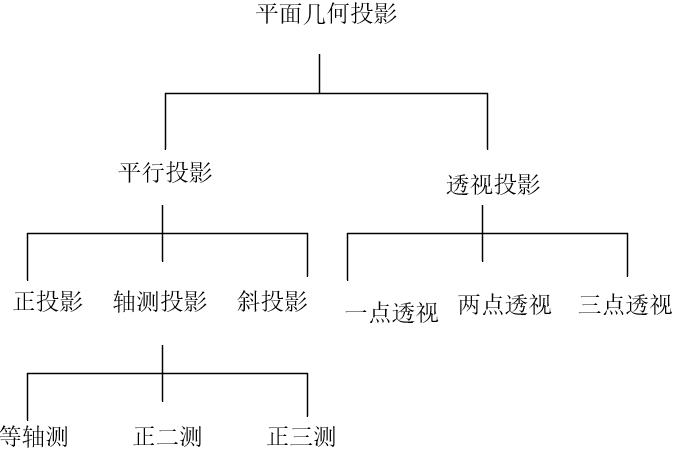
\includegraphics[scale=1.0]{touying.png}
	\end{center}
	\paragraph{4.为什么Phong着色方法绘制的图像很光滑}
	\paragraph{答:}Phong着色方法,通过对多边形顶点的法矢量进行线性插值来获得其内部各点,然后基于法矢量,采用Phong光照明模型进行明暗计算,又称为法向量插值着色方法。由于对法向量进行插值,较好的避免了Mach带效应。
	\paragraph{5.试述基于图像的隐藏面消除算法与基于对象的隐藏面消除算法的概念和特点}
	\paragraph{答:}(1)图像精度算法和对象精度算法各自的概念;page324
	\par (2)图像精度算法是基于显示设备的分辨率来判断每个像素的可见性,对象精度算法是基于对象定义的精度来判断每个对象的可见性;
	\par (3)图像精度在计算可见性时存在走样问题,对象精度算法不存在此问题;
	\par (4)一般来说,图像精度算法绘制速度更快,对象精度算法绘制的精度更高。
	\paragraph{6.几何连续的概念是什么?试举例有什么用?}
	\paragraph{答:}几何连续;倒数方向相同,但模不同,即切线方向相同,但大小不同。
	\par 在画图程序里,用户可交互的修改切线大小,保留其方向不变。

	\section{论述题}
	\paragraph{1.请描述人类视觉系统是如何得出一个简单有用的颜色模型的}
	\paragraph{参考解答:}(8')
	\par (2')一种可见的颜色可以由一个波长的函数C(d)来表征,这里d的取值范围大致从350-780nm。C(d)在可见光谱的范围内一个给定波长d处的值给出了颜色中那个波长分量的强度。
	\par (6')人类视觉系统有三类视锥细胞负责颜色视觉。因此,对于一种给定的颜色,我们的大脑接受到的不是完整分布的C(d),而是三类视锥细胞对颜色的响应值。这三个响应值叫三刺激值。这样,颜色被归结为三个数,由此引出了三色理论的基本原则,如果两种颜色的三刺激值相同,那么人眼就无法把它们区分开。
	\par 原则上,只需要三种原色就可以获得人类观察者可以看到的颜色。通过调节每种原色的强度来生成一种颜色。

	\paragraph{2.请从测量过程和触发器之间的关系描述输入设备获得一个设备的测量数据的三种不同模式}
	\paragraph{参考解答:}(8')
	\par (2')请求模式,采样模式和事件模式 page86
	\par (6')在请求模式(request mode)下,除非设备被触发,否则设备的测量数据不会返回给程序。
	\par 在采样模式(sample mode)下,输入是即时的。只要用户程序中遇到了函数调用,就把测量数据返回给程序,因此不需要触发器。
	\par 第三种模式是事件模式(event mode),该模式可以处理其他交互模式。
	\par 事件队列
	\par 回调函数
	\newpage
	\paragraph{3.请描述齐次坐标的几何意义与作用}
	\paragraph{参考解答:}(8')
	\par (2')齐次坐标的几何意义可以从许多角度来解释。page117
	\par (6')齐次坐标对三维空间中点和向量的表示都是四维的。在由(v1,v2,v3,Po)确定的标架中,任一点P可以唯一地表示为$p=\begin{bmatrix}
	\alpha_{1}\\\alpha_{2}\\\alpha_{3}\\1
	\end{bmatrix}$
	\par 任一向量w可以写成下面的形式$w=\begin{bmatrix}
	\delta_{1}\\\delta_{2}\\\delta_{3}\\0
	\end{bmatrix}$
	\par 借助齐次坐标表现成矩阵相乘的形式
	\par 现代硬件直接实现了齐次坐标的运算,而且利用并行机制来提高计算速度。

	\paragraph{4.请描述观察坐标系的建立}
	\paragraph{参考解答:}(8')
	\par (2')
	\begin{center}
		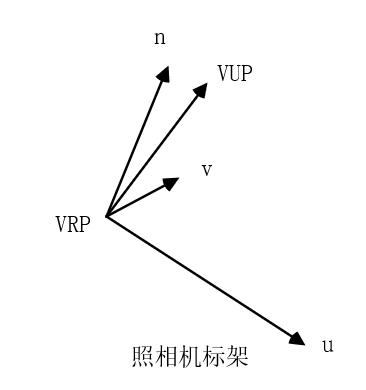
\includegraphics[scale=1.0]{zhaoxiangji.png}
	\end{center}
	\par (6')把照相机放到一个叫做观察参考点VRP的位置,接下来指定照相机的方向,可以把这个指定分成两部分:指定观察平面法向量VPN和指定观察正向量VUP,VPN给出了投影平面的方向。投影平面的方向并没有确定在照相机看来哪个方向是向上的方向。为了获得方向向上的向量v,我们把VUP向量投影到观察平面。借助投影,用户不需要计算出一个位于投影平面内的的向量,任何不平行于v的向量也可以被指定为VUP。向量v与n正交。我们可以用叉积获得与这两个向量都正交的第三个向量u。这个新的正交坐标系通常被称为观察坐标系或者u-v-n坐标系。
	\paragraph{5.请描述规范化投影技术}
	\paragraph{参考解答:}(8')
	\par (4')投影的规范化,先把对象边形,是得边形后的对象的正交投影图与原来想要得到的投影图相同,这样就把所有的投影都化为正交投影。p179
	\par (4')投影规范化由投影变换矩阵来实现。
	\par 例子:(1个即可)
	\par 正投影变换矩阵 p180
	\par 斜投影变换矩阵
	\par 简单的透视投影变换矩阵
	
	\section{计算题}
	\paragraph{1.请使用Bresenham中点画线算法生成直线段P1(1,0) P2(8,5),要求写出生成过程中像素点的坐标和判别式的值}
	\paragraph{参考答案:}(10') p318
	\par $\Delta y=y2-y1=5-0=5, \Delta x=x2-x1=8-1=7$
	\par $incrE=2\Delta y=10,incrNE=2(\Delta y-\Delta x)=-4$
	\par 初始条件,$d=2\Delta y-\Delta x=10-7=3$
	\par i xi yi d
	\par 1 1 0 3
	\par 2 2 1 -1
	\par 3 3 1 9
	\par 4 4 2 5
	\par 5 5 3 1
	\par 6 6 4 -3
	\par 7 7 4 7
	\par 8 8 5
	
	\paragraph{2.如图所示,风筝放飞前位于坐标A(10,2)、B(9,1)、C(9,0)、D(11,0)、E(11,1)且其中心点为P(10,1),放飞后中心点变为Q(3,5),且围绕中心点法线逆时针旋转45度,并因越飞越远使得尺寸缩小为原来的一半,请写出风筝放飞前后的组合变换矩阵,并求A、B、C三点变换后A'、B'、C'的坐标。}
	\begin{center}
		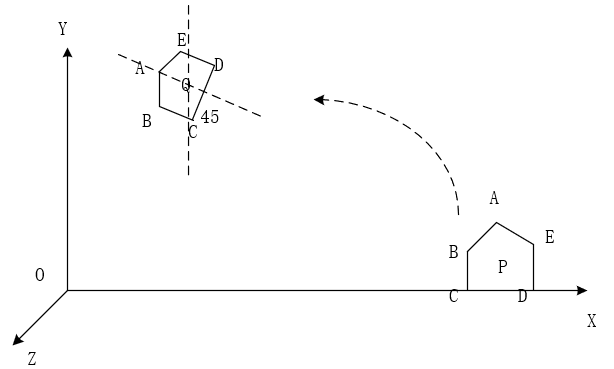
\includegraphics[scale=1.0]{zuobiao.png}
	\end{center}
	\paragraph{参考答案:}(10')
	\par 首先把五边形ABCDE平移使得中心点P与坐标原点重合,然后把五边形绕z轴旋转45度,接着把五边形做缩放变换使其尺寸变为原来的一半,最后平移五边形中心点到Q点。此变换序列可以用以下矩阵的乘积表示:
	\par $TM=T(qx,qy)S()R(\theta)T(-px,-py)$
	\begin{equation*} 
	=\begin{bmatrix}
	1&0&qx\\
	0&1&qy\\
	0&0&1
	\end{bmatrix}\begin{bmatrix}
	\frac{1}{2}&0&0\\
	0&\frac{1}{2}&0\\
	0&0&1
	\end{bmatrix}\begin{bmatrix}
	cos\theta&-sin\theta&0\\
	sin\theta&cos\theta&0\\
	0&0&1
	\end{bmatrix}\begin{bmatrix}
	1&0&-px\\
	0&1&-py\\
	0&0&1
	\end{bmatrix}
	\end{equation*}
	\par 其中,px=10,py=1,qx=3,qy=5,$\theta$=45
	\par 基于复合变换矩阵,计算P2与P3变换后的结果:
	\par $A'=TM\cdot A, B'=TM\cdot B, C'=TM\cdot C$
	
	\paragraph{3.设有两段三次Bezier曲线P(u)和R(v),其中曲线P的四个控制点为P0(0,0,0),P1(1,2,--1),P2(2,3,1),P3(3,0,0)。而曲线R的四个控制点为R0(3,0,0),R1(4,-2,1),R2(5,-2,-1),R3(6,0,0)。请写出曲线P(u)的表达式并计算参数u为0.5时的值,并且判断曲线P(u)和R(v)是否为C0与C1连续。}
	\paragraph{参考答案:}(10')
	\par $M_{B}=\begin{bmatrix}
	1&0&0&0\\
	-3&3&0&0\\
	3&-6&3&0\\
	-1&3&-3&1
	\end{bmatrix}$
	\par $P(u)=\begin{bmatrix}
		1&u&u^{2}&u^{3}
	\end{bmatrix}M_{B}\begin{bmatrix}
	P_{0}&P_{1}&P_{2}&P_{3}
	\end{bmatrix}^{T}$
	\par $\begin{bmatrix}
	1&u&u^{2}&u^{3}
	\end{bmatrix}\begin{bmatrix}
	1&0&0&0\\
	-3&3&0&0\\
	3&-6&3&0\\
	-1&3&-3&1
	\end{bmatrix}\begin{bmatrix}
	P_{0}\\
	P_{1}\\
	P_{2}\\
	P_{3}
	\end{bmatrix}$
	\par 将u=0.5代入计算P(0.5)
	\par $P'(1)=3(P_{3}-P_{2})=3(1,-3,-1)$而$R'(0)=3(R_{1}-R_{0})=3(1,-2,1)$
	\par 由于$P_{3}=R_{0}$,因此曲线P(u)和R(v)是C0连续。
	\par 由于$P'(1)\neq R'(0)$,因此曲线P(u)和R(v)不是C1连续。

\end{document}